\documentclass[12pt]{article}    % <--- 12pt font
\usepackage[margin=1in]{geometry}% <--- 1 in margin
\linespread{1.5}
\usepackage[utf8]{inputenc}
\usepackage{natbib}
\usepackage{setspace} 
\usepackage{graphicx}
\usepackage{lscape}
\usepackage{tabularx}\usepackage{subfigure}
\usepackage{lipsum}
\usepackage{subcaption}
\usepackage[]{graphicx} 
\usepackage{makecell}
\usepackage{tikz}
\usepackage[%  
    colorlinks=true,
    pdfborder={0 0 0},
    linkcolor=blue,
    urlcolor=red,
    linktoc=all,
    citecolor=blue
]{hyperref}
\usepackage{colortbl}
\usepackage[gen]{eurosym}
\usepackage{caption}
\DeclareCaptionLabelFormat{AppendixTables}{A.#2}
\usepackage[title]{appendix}
\usepackage{booktabs}
\usepackage{graphicx}
\graphicspath{ {./images/} }
\usepackage{cleveref}
\usepackage{xcolor}
\newcommand{\MYhref}[3][blue]{\href{#2}{\color{#1}{#3}}}%
\usepackage{pdfpages}
\usepackage[round]{natbib} 
\usepackage[capposition=top]{floatrow}
\usepackage{floatrow}
\usepackage{rotating}
\usepackage[edges]{forest}
\usepackage{blkarray}
\usepackage{enumitem} 
\usepackage[colorinlistoftodos]{todonotes}
\usepackage{lipsum} % dummy text for the MW
\usepackage{xcolor}
\usepackage{tabularx}
\usepackage{rotating}
\usepackage{hyperref}
\usepackage{breqn}
\hypersetup{colorlinks = true, linkcolor = blue }
\renewcommand{\baselinestretch}{1.5}
\usepackage[english]{babel}
\usepackage{enumitem}
\usepackage{xspace}
\newcommand\nd{\textsuperscript{nd}\xspace}
\newcommand\rd{\textsuperscript{rd}\xspace}
\newcommand\nth{\textsuperscript{th}\xspace} %\th is taken already
\usepackage{array}
\usepackage{blindtext}
\usepackage[final]{pdfpages}
\usepackage[T1]{fontenc}
\usepackage{mathtools}
\usepackage{hyperref}
\usepackage{breqn}
\hypersetup{colorlinks = true, linkcolor = blue }
\renewcommand{\baselinestretch}{1.5}
\usepackage[english]{babel}
\usepackage{newtxtext,newtxmath}
\usepackage{geometry,mathtools}
\usepackage{amsmath}
\DeclareUrlCommand\url{\color{blue}}
\newcommand{\underwrite}[3][]{
  \genfrac{}{}{#1}{}{\textstyle #2}{\scriptstyle #3}
}
\usepackage{hyperref}
\newcommand{\footremember}[2]{%
    \footnote{#2}
    \newcounter{#1}
    \setcounter{#1}{\value{footnote}}%
}
\newcommand{\footrecall}[1]{%
    \footnotemark[\value{#1}]%
}

\usepackage[gen]{eurosym}
\usepackage{caption}
\DeclareCaptionLabelFormat{AppendixTables}{A.#2}
\usepackage[title]{appendix}
\usepackage{booktabs}
\graphicspath{ {./images/} }
\usepackage[runin]{abstract}
\setlength{\abstitleskip}{-\parindent} 
\setlength{\absleftindent}{0pt} 
\setlength{\absrightindent}{0pt}

\renewcommand{\abstractnamefont}{\normalfont\bfseries} 
\renewcommand{\abstracttextfont}{\normalfont} 
\abslabeldelim{:\quad} 
\usepackage{adjustbox}
\usepackage{subcaption}
\usepackage{subfig,graphicx}
\usepackage{verbatim}
\usepackage[capposition=top]{floatrow}
\usepackage{floatrow}
\usepackage[edges]{forest}
\usepackage{blkarray}
\usepackage{enumitem} 
\usepackage[colorinlistoftodos]{todonotes}
\usepackage{lipsum} 
\usepackage{xcolor}
\usepackage{tabularx}
\usepackage{rotating}
\usepackage{hyperref}
\usepackage{breqn}
\hypersetup{colorlinks = true, linkcolor = blue }
\renewcommand{\baselinestretch}{1.5}
\usepackage[english]{babel}
\usepackage{enumitem}
\usepackage{array}
\usepackage{blindtext}
\usepackage[final]{pdfpages}
\usepackage{hyperref}
\usepackage[T1]{fontenc}
\usepackage{mathtools}
\usepackage{newtxtext,newtxmath}
\usepackage{geometry,mathtools}
\usepackage{amsmath}



\setlength{\droptitle}{-7em}
\title{\large Bring  Together What Belongs Together: \\The Case of Divided Cities in Europe}


\author{Ketevani Kapanadze\textsuperscript{\textdagger}}
\date{\small \today}

\begin{document}

\maketitle

\renewcommand{\thefootnote}{\textdagger} % Change footnote marker to †
\hypersetup{urlcolor=blue} % Ensure hyperlinks are blue
\footnotetext{\textcolor{blue}{\footnotesize \href{ketevani.kapanadze@eruni.org}{ketevani.kapanadze@eruni.org}}, European Research University (ERUNI), Politických vězňů 1419/11 Prague.
\vspace{0.5cm}
\\I am very grateful to Mariola Pytlikova for guidance and encouragement. Thanks to Christian Ochsner, Nikolaus Wolf, Gabriel Alhfeildt, Sebastian Ottinger, Paolo Zacchia, Stepan Mikula, Federico Trionfetti, Lydia Assouad, Christina Felfe, Lukas Makovsky, and Irakli Barbakadze for their constructive comments and suggestions. I also want to extend my gratitude to  Christian Lessmann, Felix Roesel, Anna Kremer and all participants in the Regional Economics workshop at the ifo Institute for all valuable discussions. I am very grateful to ANET Lab and KRTK for inviting to the seminar series - I  appreciate all the received feedback, special thank to Balazs Lengyel and Zoltan Elekes.  I greatly appreciate all the help I received during the academic job market: from Deborah Novakova and the academic skills center at CERGE-EI. This paper was supported by the Czech Science Foundation (GACR) grant No. 20-31615S and the NPO "Systemic Risk Institute" number LX22NPO5101, funded by European Union - Next Generation EU (Ministry of Education, Youth and Sports, NPO: EXCELES). All remaining errors are mine. }
\renewcommand{\thefootnote}{\arabic{footnote}} % Reset footnote marker to default for the rest of the document



\maketitle
\begin{abstract}
\footnotesize
\par Do spatial concentrations of economic activities have deep historical roots in Europe? This paper explores a unique quasi-natural experiment of opening borders within cities that were historically a single urban entity and were divided due to border shifts following major historical conflicts. After inter-city borders were opened, I find that local economic activities, measured by remotely sensed nightlight, became more concentrated close to the pre-division city centers. This raises an important question, what type of border opening is more important in spurring agglomeration, the free movement of goods or of people? When looking into potential mechanisms behind the impact, using national business register databases, I find that proximity to former historical centers is more prominent, particularly after allowance of the free movement of people as a part of the Schengen agreement in 2008, whereas gaining broader market access following the 2004 EU enlargement is less important. I account for two main channels. First, I show that firms in the consumption sectors are more exposed to the free movement of people and are more likely to start operating closer to historical city centers than are firms in the production sectors, which are less affected by local market potentials. Second, I show that cities in which cultural and language differences are not barriers to cross-border cooperation are more influenced by the free movement of people than cities where these barriers still exist. Hence, spatial agglomerations near pre-division city centers are more apparent in almost borderless cities.
\vspace{}
\par \textbf{Keywords}: Divided cities, borders, historical centre, nightlights, registered firms, Schengen
%\par  \textbf{JEL Codes:}  R12, N14, E65 
\end{abstract}

\newpage

\section{Extended Abstract}


\par This paper aims to address the challenge of finding exogenous variations that are uncorrelated with locational fundamentals by examining a unique quasi-natural setting of removing borders along divided European historical border cities that were once united in the past. I show that local economic activities, measured by remotely sensed nighttime lights (NTL) and by the number of newly established firms, concentrated denser and closer to the pre-division 20th-century centers as Schengen has abolished border barriers and facilitated the free movement of people across Europe. This paper
takes a comprehensive and multinational perspective by examining 22 European historical cities in 10 European countries. It aims to provide a high-resolution analysis by utilizing localized data specific to each historically divided city.
 
\par Divided historical border cities in Europe were one urban unit before the World Wars, and after major international border shifts, cities came apart. For example, the historical German city Frankfurt (Oder) was divided into an East German city - Frankfurt (Oder), and a Polish city - Slubice; the latter was a German suburb called Dammvorstadt until 1945. The lack of cooperation between East Germany and Poland during the communist era created obstacles to cross-border interactions and economic integration. The division of Frankfurt (Oder) and Slubice resulted in economic activities being dispersed away from the pre-division centers due to the restricted movement and limited cooperation between the two separated cities. However, the Eastern enlargement of the European Union in 2004 and Poland's subsequent entry into the Schengen Area in 2008 further facilitated the step-wise development of cross-border cooperation and the free movement of goods, people, and services between the two cities\footnote{It was difficult to freely cross the internal borders between the cities until Poland joined the Schengen Area in  2008.}. After joining Schengen, all border barriers were lifted, enabling divided cities to work together freely once again. I show that economic activities began to re-concentrate toward the pre-division centers. My results suggest that integration policies can bring together what historically belongs together, internal city structures change, and the concentration of economic activities shifts to historical centers. 


\par My paper builds on the large literature on the effect of quasi-natural experiments on the location of economic activity within cities, particularly from a historical perspective. One strand of literature has explored technological inventions in transportation or transportation extensions, e.g.,  \cite{baum2005effects} examines the effects of urban rail transit expansions in sixteen major U.S. cities; \cite{brooks2019vestiges} study the period when streetcars dominated urban transit in Los Angeles county and explore the effects of transportation infrastructure on economic concentration; \cite{heblich2020making} focus on the invention of steam railways in London and analyzes the impacts of transportation innovations on economic clustering. Another strand of literature studies the role of historical policies and historical events within cities, including \cite{arzaghi2008networking}, which investigated the factors influencing the spatial distribution of advertising agencies in Manhattan. They focused on the role of networking externalities and agglomeration economies in shaping the location decisions of advertising agencies; \cite{rossi2010housing} examined the impact of urban revitalization policies on housing externalities in Richmond, Virginia. They focused on concentrated revitalization programs that aimed to improve specific neighborhoods within the city, and \cite{ahlfeldt2015economics} examined the economic consequences of the division and subsequent reunification of Berlin, Germany. It seems as if there is some consensus on understanding the sources and dynamics of economic concentration within the cities. However, the area is still under-researched. The existing literature often focuses on specific cities, which may limit the generalizability of the findings. Each city has its unique characteristics, historical background, and economic structure, which can lead to different channels of agglomeration forces at play. 


\par This paper contributes to the stream of literature by exploring a unique quasi-natural experiment of opening borders within cities, which used to be  one city in the past and were divided following major historical conflicts. The closest to my work is a study by \cite{ahlfeldt2015economics}, where authors study how the reunification of Berlin affected the city’s economic landscape, including
the role of historical city centers and their transformation in the post-reunification era.
My central contribution is assessing border effects for a different type of border (e.g., with its different historical and institutional circumstances) than the imposition and removal of the Iron Curtain. In contrast to their study, my paper which studies cities that were split into two different countries with different languages and cultures, allows me to shed some light on different mechanisms and channels. 


\par My paper's setting of multiple border cities and detailed NTL and business register data allows me to study different underlying economic mechanisms  and channels of agglomeration forces, something that has not been studied yet, to the best of my knowledge. The paper has the main findings in the following three aspects. 


\par First, the implementation of the free movement of people policy in 2008 had a significant impact on reorienting economic and human activities towards pre-division city centers. However, the "borderless market" or free movement of goods, services, and capital in 2004 did not have the same effect. This indicates that factors other than the movement of goods and capital, such as the direct engagement and interaction of people, play a more significant role in driving economic concentration near historical centers.


\par Second, city heterogeneity allowed me to investigate the role of language and cultural closeness between divided city pairs. While historical centers tend to be hubs of social activities, language similarity should enhance participation and integration into cross-national networks.  Therefore, I show that businesses are more likely to concentrate on areas where they can effectively communicate and engage with the local and foreign markets. I show that economic activities concentrate closer to former historical centers in city pairs where lexical similarities are high between languages in divided cities and cultural and language differences are not barriers to cross-border cooperation. 


\par Third, using a data set on registered firms in divided border cities, I show that the consumption-oriented sectors concentrate near pre-division centers.  Firms in the consumption sector facilitate greater interaction and connectivity among local and foreign people. I show that  restaurants, cafes, and cultural and entertainment venues started operating in a close radius of former historical centers after removing all types of borders in divided cities. Customers from both sides of the formerly united city can come to these areas, leading to increased physical movement and social interactions. This increased human mobility could create shared spaces, fostering a sense of togetherness and community within the divided city.

\par This paper also contributes to the European integration literature. While there has been researched on the broader impacts of EU integration on regional development and urbanization patterns \textit{across} European cities (\citealp{Brakman2012}; 
\citealp{brulhart2018trade}; 
\citealp{Heider2019}), the concentration and spatial distribution of economic activities \textit{inside} cities in the course of European integration have not been studied before. 







\begin{figure}[H] \hypertarget{Figure 2.1}{}
\renewcommand\thefigure{2.1} 
\RawCaption{\caption{Divided Border Cities in Europe} }\vskip\captionskip
\floatbox[{\captop}]{figure}[\FBwidth]
    {}
   {
    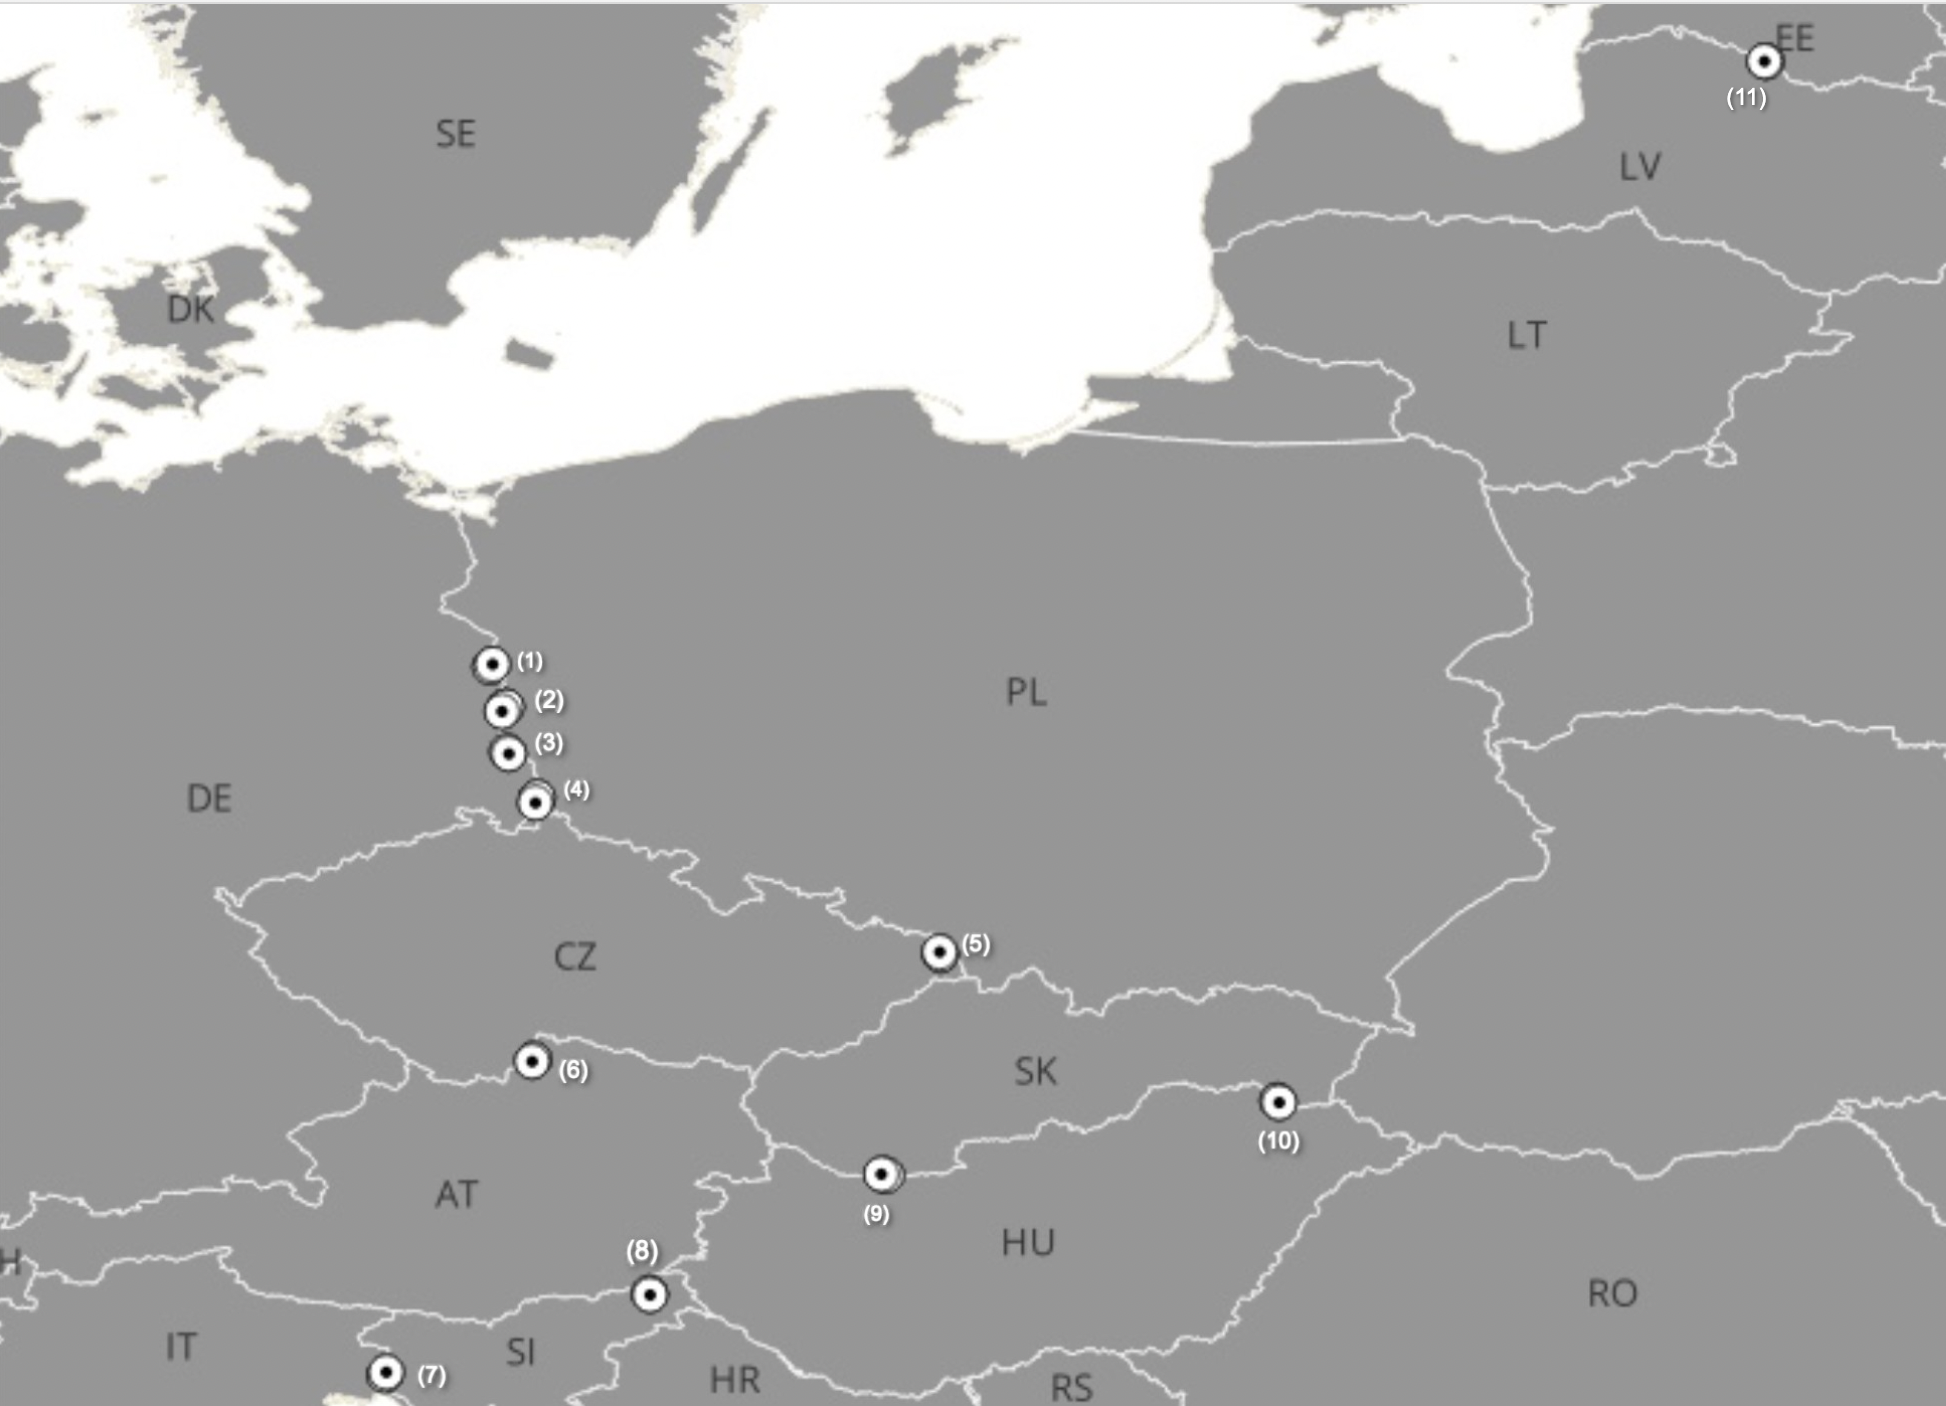
\includegraphics[scale=0.45]{photos/dividedcities.png}
    \floatfoot{ 
\scriptsize 
\textit{Source:} Author's elaboration based on GISCO shapefiles. \\\textit{Notes}: Circles on the map illustrate 22 divided cities in 10 European countries, i.e., Germany (DE), Poland (PL), Czechia (CZ), Slovenia (SI), Slovakia (SK), Austria (AT), Hungary (HU), Italy (IT), Estonia (EE), and Latvia (LV). Divided cities  are (1) Frankfurt (Oder) - Slubice, (2) Zgorzelec - Gorlitz, (3) Guben - Gubin, (4) Leknica - Bad Muskau, (5) Ceske Teshin - Cieszyn, (6) Gmund - Ceske Velenice, (7) Nova Gorica - Gorizia, (8) Bad Radkersburg - Gornja Radgona, (9) Komarom - Komarno, (10) Satoraljaujhely - Slovenske Nové Mesto, (11) Valga - Valka}}
\end{figure}


\begin{figure}[H] \hypertarget{Figure 2.2}{}
\renewcommand\thefigure{2.2}
\RawCaption{\caption{Three Phases of Hypothesis Framework}}\vskip\captionskip
\floatbox[{\captop}]{figure}[\FBwidth]
    {}
   {
    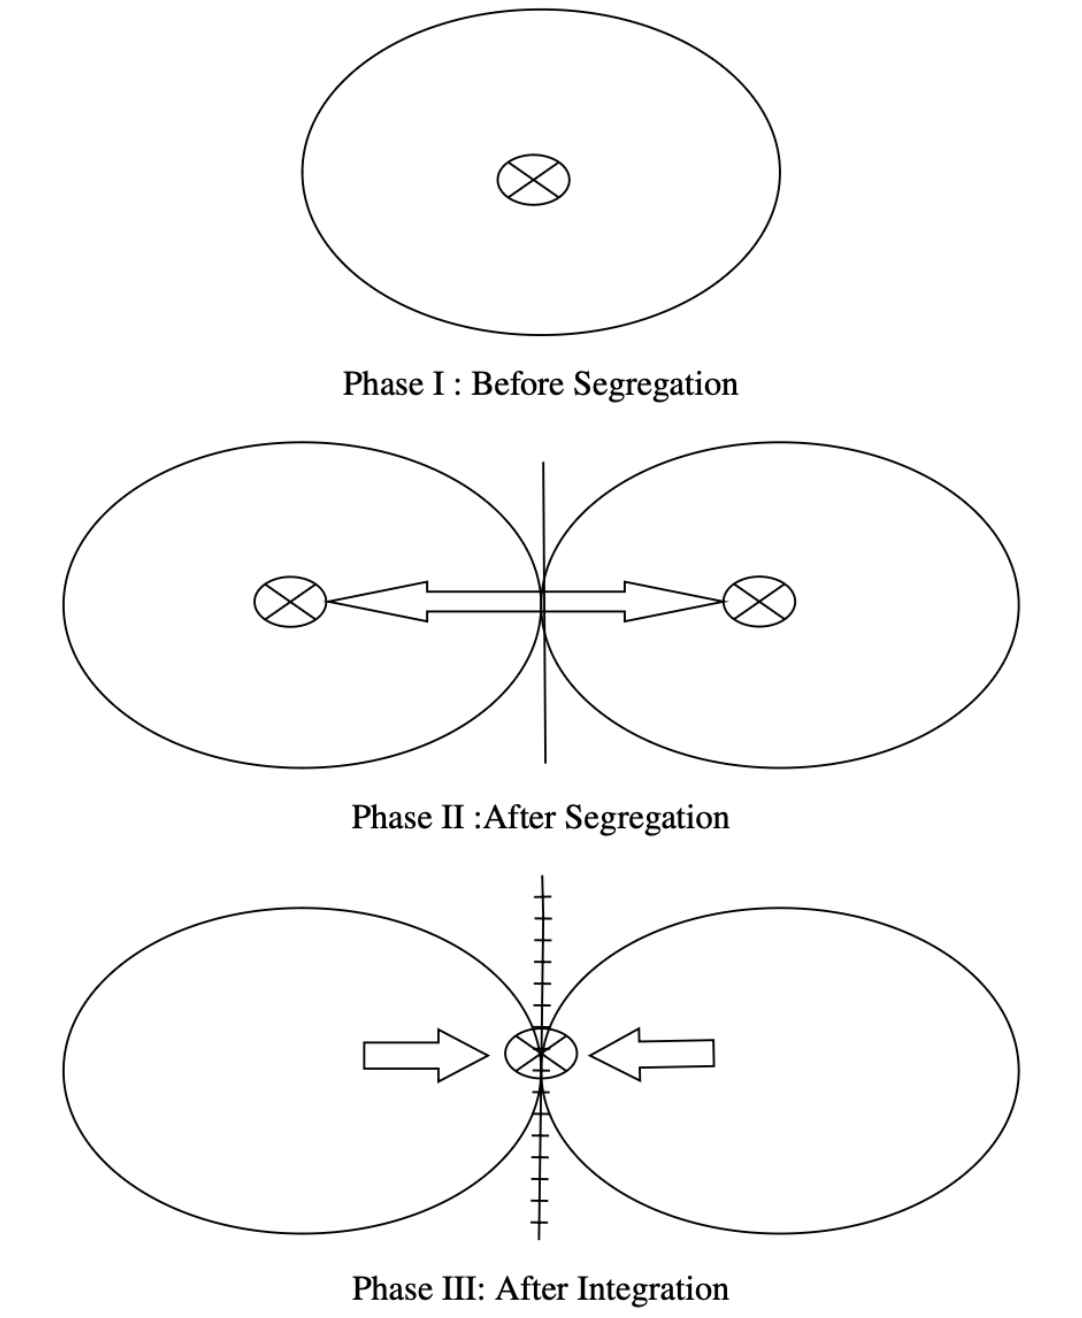
\includegraphics[scale=0.4]{photos/hypoframe.png}
    \floatfoot{ 
\scriptsize \textit{Notes:} Dashed circles in the circles represent 20th historical city centers. Arrays denote in which direction economic activities move. The solid line represents emerged border. The dashed line represents a lifted intra-city or state border.}}
\end{figure}


\newpage
\bibliographystyle{apalike}
\bibliography{reference}


\end{document}
